% The four HPS decay modes considered at analysis level, for Chapter II (fig:tau_DMs).
% Same style as the tau_h signatures of Chapter III (fig:tau_fakes).
% Adapted from https://tikz.net/tau_decay/ (Izaak Neutelings, CC BY-SA 4.0).
\documentclass[11pt,border=2pt]{standalone}
\usepackage[T1]{fontenc}
\usepackage{cochineal}
\usepackage[cochineal]{newtxmath}
\usepackage{tikz}
\usetikzlibrary{decorations.markings,decorations.pathmorphing}
\tikzset{>=latex}

% vertical custom shading (for the shower cones)
% https://tex.stackexchange.com/questions/191735
\makeatletter
\tikzset{vertical custom shading/.code={%
  \pgfmathsetmacro\tikz@vcs@middle{#1}
  \pgfmathsetmacro\tikz@vcs@bottom{\tikz@vcs@middle/2}
  \pgfmathsetmacro\tikz@vcs@top{(100-\tikz@vcs@middle)/2+\tikz@vcs@middle}
  \pgfdeclareverticalshading[tikz@axis@top,tikz@axis@middle,tikz@axis@bottom]{newaxis}{100bp}{%
    color(0bp)=(tikz@axis@bottom);
    color(\tikz@vcs@bottom bp)=(tikz@axis@bottom);
    color(\tikz@vcs@middle bp)=(tikz@axis@middle);
    color(\tikz@vcs@top bp)=(tikz@axis@top);
    color(100bp)=(tikz@axis@top)}
    \pgfkeysalso{/tikz/shading=newaxis}
  }
}
\makeatother
\tikzset{
  ->-/.style={decoration={markings,mark=at position .7 with {\arrow{>}}},postaction={decorate}},
  photon/.style={decorate,decoration={snake,segment length=5,amplitude=1.1}},
  mycone/.pic={
    \shadedraw[top color=white,bottom color=black!50,shading angle=50,vertical custom shading=10]
      (-0.4,0.99) -- (0,0) -- (0.4,0.99);
    \shadedraw[top color=white,bottom color=black!20,shading angle=90]
      (0,1) ellipse (0.4 and 0.12);}
}

\begin{document}
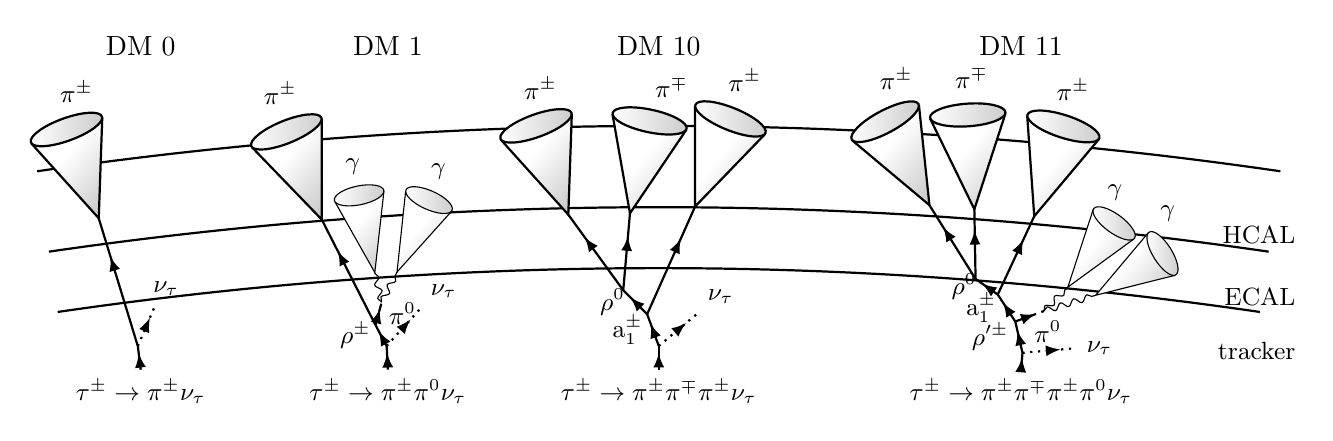
\begin{tikzpicture}[scale=0.43,every node/.style={font=\small}]
  \def\R{120}     % inner radius of the arcs
  \def\hca{8.3}   % half central angle
  \def\tracker{3}
  \def\ECAL{4.8}
  \def\HCAL{7.2}
  \pgfmathsetmacro\hclmax{(\R+\HCAL)*sin(\hca)}

  % detector layers
  \foreach \r in {\tracker,\ECAL,\HCAL}{
    \draw[thick] (0,\r) arc (90:90-\hca:\R+\r) (0,\r) arc (90:90+\hca:\R+\r);
  }
  % layer names at the right end, following the curvature of the arcs
  \node[above left] at ({1.04*\hclmax},0.0) {tracker};
  \node[above left] at ({1.04*\hclmax},1.62) {ECAL};
  \node[above left] at ({1.04*\hclmax},3.45) {HCAL};

  % decay mode of each decay, above the detector
  \foreach \x/\dm in {-15.3/{DM $0$},-8.0/{DM $1$},0.0/{DM $10$},10.7/{DM $11$}}
    \node[font=\normalsize] at (\x,9.55) {\dm};

  % ---------------- DM 0: one prong ----------------
  \begin{scope}[shift={(-15.3,0)},rotate=7]
    \node[below] at (0,0) {$\tau^\pm\to\pi^\pm\nu_\tau$};
    \draw[->-,thick] (0,0) -- (0,0.7) coordinate (tau);
    \draw[->-,dotted,thick,rotate=-30] (tau) --+ (0,1.3) node[right=4pt,above] {$\nu_\tau$};
    \draw[->-,thick,rotate=10] (tau) --+ (0,3.95) node[left=8,above=38] {$\pi^\pm$}
      pic[rotate=20,scale=1.2] {mycone};
  \end{scope}

  % ---------------- DM 1: one prong plus strip ----------------
  \begin{scope}[shift={(-8.0,0)},rotate=3]
    \node[below] at (0,0) {$\tau^\pm\to\pi^\pm\pi^0\nu_\tau$};
    \draw[->-,thick] (0,0) -- (0,0.7) coordinate (tau);
    \draw[->-,dotted,thick] (tau) --+ (45:1.5) node[above right] {$\nu_\tau$};
    \draw[->-,thick] (tau) --+ (115:0.7) coordinate (rho) node[midway,left] {$\rho^\pm$};
    \draw[->-,thick] (rho) --+ (114:3.5) node[left=15,above=38] {$\pi^\pm$}
      pic[rotate=22,scale=1.2] {mycone};
    \draw[->-,densely dashed,thick] (rho) --+ (72:0.7) coordinate (pion0) node[midway,right] {$\pi^0$};
    \draw[photon] (pion0) --+ (100:0.9) node[left=8,above=32] {$\gamma$}
      pic[rotate=11.5,xscale=0.8] {mycone};
    \draw[photon] (pion0) --+ (60:1.0) node[right=15,above=30] {$\gamma$}
      pic[rotate=-24,xscale=0.8] {mycone};
  \end{scope}

  % ---------------- DM 10: three prongs ----------------
  \begin{scope}[shift={(0.0,0)},rotate=0]
    \node[below] at (0,0) {$\tau^\pm\to\pi^\pm\pi^\mp\pi^\pm\nu_\tau$};
    \draw[->-,thick] (0,0) -- (0,0.7) coordinate (tau);
    \draw[->-,dotted,thick] (tau) --+ (40:1.5) node[above right] {$\nu_\tau$};
    \draw[->-,thick] (tau) --+ (110:1.0) coordinate (a1) node[midway,left] {a$_1^\pm$};
    \draw[->-,thick] (a1) --+ (135:1.0) coordinate (rho) node[midway,left] {$\rho^0$};
    \draw[->-,thick] (rho) --+ (126:2.76) node[left=10,above=38] {$\pi^\pm$}
      pic[rotate=20,scale=1.2] {mycone};
    \draw[->-,thick] (rho) --+ (85:2.28) node[right=15,above=38] {$\pi^\mp$}
      pic[rotate=-12,scale=1.2] {mycone};
    \draw[->-,thick] (a1) --+ (66:3.48) node[right=18,above=38] {$\pi^\pm$}
      pic[rotate=-22,scale=1.2] {mycone};
  \end{scope}

  % ---------------- DM 11: three prongs plus strip ----------------
  \begin{scope}[shift={(10.7,0)},rotate=-5]
    \node[below] at (0,0) {$\tau^\pm\to\pi^\pm\pi^\mp\pi^\pm\pi^0\nu_\tau$};
    \draw[->-,thick] (0,0) -- (0,0.5) coordinate (tau);
    \draw[->-,dotted,thick] (tau) --+ (10:1.6) node[right] {$\nu_\tau$};
    \draw[->-,thick] (tau) --+ (108:0.95) coordinate (rhop) node[midway,left] {$\rho'^\pm$};
    \draw[->-,thick] (rhop) --+ (128:0.95) coordinate (a1) node[midway,left] {a$_1^\pm$};
    \draw[->-,thick] (a1) --+ (150:0.8) coordinate (rho) node[midway,left] {$\rho^0$};
    \draw[->-,thick] (rho) --+ (127:2.57) node[left=12,above=38] {$\pi^\pm$}
      pic[rotate=28,scale=1.2] {mycone};
    \draw[->-,thick] (rho) --+ (96:2.06) node[left=1,above=40] {$\pi^\mp$}
      pic[rotate=4,scale=1.2] {mycone};
    \draw[->-,thick] (a1) --+ (70:2.55) node[right=14,above=38] {$\pi^\pm$}
      pic[rotate=-18,scale=1.2] {mycone};
    \draw[->-,densely dashed,thick] (rhop) --+ (25:0.9) coordinate (pion0) node[midway,below right=-2pt] {$\pi^0$};
    \draw[photon] (pion0) --+ (50:1.0) node[right=17,above=28] {$\gamma$}
      pic[rotate=-36,xscale=0.8] {mycone};
    \draw[photon] (pion0) --+ (22:1.6) node[right=26,above=23] {$\gamma$}
      pic[rotate=-58,xscale=0.8] {mycone};
  \end{scope}
\end{tikzpicture}
\end{document}
